\documentclass[10pt]{article}
\usepackage[margin=1cm]{geometry}
\usepackage{setspace}
\setstretch{0.9}

\usepackage{enumitem}\setlist[itemize]{topsep=0pt}
\usepackage{amssymb}
\usepackage{amsmath}
\usepackage{fancybox}
\usepackage{graphicx}
\usepackage{fancyvrb}
\usepackage[most]{tcolorbox}


\usepackage{cse571}
\raggedright
\pagestyle{empty}
\pagenumbering{gobble}
\begin{document} \noindent

\section*{cse571 midterm review}

bayseian network conditional indepedence: use markov blanket for belief propagation
\hspace{2em}
\begin{minipage}[b]{0.6\textwidth}
    for nodes in $\mathbf{A} \subset \mathbf{N}$ where
    \begin{itemize}[leftmargin=1em, itemsep=-0.3em]
        \item[] $\mathbf{N}$:= universe of all nodes in network
        \item[] $\mathbf{B}$:= $blanket(\mathbf{A})$, markov blanket (neighbours) of nodes in $\mathbf{A}$
        \item[] $\mathbf{C}$:= $\mathbf{N}\setminus(\mathbf{A} \cup \mathbf{B})$, nodes not in $\mathbf{A}$ or $\mathbf{B}$
    \end{itemize}
    conditional indepedence: $(\mathbf{A}\condind \mathbf{C})\ |\ \mathbf{B}$\\
\end{minipage}
\begin{minipage}[b]{0.2\textwidth} \footnotesize
    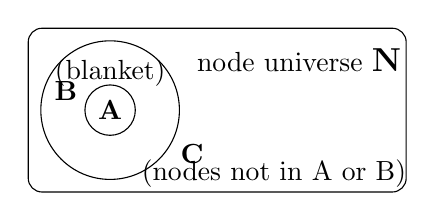
\begin{tikzpicture}[scale=0.8]
        \def\setcircle{(1.4,1.4) coordinate (a) circle (0.4)}
        \def\blanket{(1.4,1.4) coordinate (b) circle (1.1)}
        \def\universe{(0.1,0.1) coordinate (u) rectangle (6.1,2.7)}
        % \begin{scope}
        %     \fill[yellow!40] \universe;
        %     \clip \blanket;
        %     \fill[magenta!40] \blanket;
        %     \clip \setcircle;
        %     \fill[cyan!50] \setcircle;
        % \end{scope}
        \draw \setcircle node at (1.4,1.4) {$\mathbf{A}$};
        \draw \blanket node at (0.7,1.7) {$\mathbf{B}$};
        \node at (1.4,2) {(blanket)};
        \draw[rounded corners=5pt] \universe node at (4.4,2.2) {node universe \large $\mathbf{N}$};
        \node at (2.7,0.7) {$\mathbf{C}$};
        \node at (4,0.4) {(nodes not in A or B)};
    \end{tikzpicture}
\end{minipage}

\begin{table}[h]
    \small
    \begin{tabular}{|c|c|c|c|c|} \hline
        rectified linear unit                                                                                           & sigmoid & hyperbolic tangent & exponential linear unit & softmax
        \\ \hline
        $relu(x) = max(0, x)$                                                                                           &
        $\sigma(x) = \displaystyle\frac{1}{1 + e^{-x}}$                                                                 &
        $tanh(x) = \displaystyle\frac{e^{x} - e^{-x}}{e^{x} + e^{-x}}$                                                  &
        $elu(x) = \begin{cases} x & x > 0 \\ \alpha(e^{x} - 1) & x \leq 0 \end{cases}$                                  &
        $softmax_i(x) = \displaystyle\frac{e^{x_i}}{\sum e^{x_k}}$
        \\
        $\displaystyle \frac{\partial}{\partial x} = \begin{cases} 1 & x > 0 \\ 0 & x \leq 0 \end{cases}$               &
        $\displaystyle \frac{\partial}{\partial x} = \sigma(x)(1: \sigma(x))$                                           &
        $\displaystyle \frac{\partial}{\partial x} = 1 - tanh^2(x)$                                                     &
        $\displaystyle \frac{\partial}{\partial x} = \begin{cases} 1 & x > 0 \\ elu(x) + \alpha & x \leq 0 \end{cases}$ &
        \\\hline
        %                                                                                                                 &         &                    &                         &
        % \rule{0pt}{5em}                                                                                                                                                                    \\ \hline
    \end{tabular}
\end{table}

\section*{week 1: intro to machine learning}

\begin{itemize}[label=\(\star\), leftmargin=1em, itemsep=-0.3em]
    \item supervised learning: model learns mapping of input to output
    \item high generalization: make accurate predictions/classifications on new/unseen data
    \item loss/cost/error function: minimize distance to target labels
    \item functional view maps inputs to outputs (vs) probabilistic view calculates conditional probability distributions based on inputs
    \item reinforcement learning: sequential decisions, explore actions and observe consequences, optimize reward/punishment (manually specified), autonomy, trial\&error, learn policy for realtime decisions
    \item RL policy: takes state as input and outputs action, can be deterministic or stochastic, maximizes expected cumulative reward over time
    \item binning: approximate joint distribution over variables, capture discrete patterns/categories, non-linear relationships, relationships with by distinct ranges/intervals rather than continuous function (regression)
    \item dimentionality reduction: manifold learning, reduce number of features (and noise, computational cost)
    \item stochastic gradient descent: update model params based on average gradient computed from mini-batch (randomly selected subset of training data), memory-efficient, adds noise to escape local minima, makes an update step for each sample
    \item qubits: quantum bits, can hold an exponential number of states using superposition (of 0 and 1) and entanglement (for parallel computation)
    \item QML rotation embedding: relatively simple to implement, uses only linear number of qubits
    \item if normalization is not performed on input data features that have higher values will influence network more, and very small values will have no effect at all - quality of learning decreases
    \item in QML, data embedding requires storing classical data in quantum states
    \item in QML, amplitude encoding  has higher qubit requirement than rotation encoding
    \item ansatz (in qml) typically refers to designing structure and layers of neural network
\end{itemize}

\section*{week 2: intro to neural networks}

\begin{itemize}[label=\(\star\), leftmargin=1em, itemsep=-0.3em]
    \item training time: depends on convergence rate
    \item early-stopping: stop training when validation loss starts increase, may require more iterations of training to find optimal model
    \item activation function: must be non-linear (eg sigmoid, tanh, ReLU, softmax), should be computationally efficient
    \item update step of gradient descent: $weight_{new} = weight_{old}: learning\_rate * gradient$, learning rate determines size of step taken in direction of gradient
    \item softmax outputs a probability distribution over multiple classes (vs) sigmoid outputs a single probability for binary classifications
    \item softmax: outputs a probability distribution over multiple classes, sum of all probabilities is 1, used for multi-class classification
    \item forward pass: input is multiplied by weights and added to bias, then passed through activation function
    \item back-propagation objective: minimize loss function to make predictions closer to target values
    \item back-propagation algorithm (for fully connected feed-forward NN): after forward passes of input produces output, calculate loss wrt output and target weight (based on loss function) and use chain rule to calculate gradient of loss function wrt weights/biases of each layer, then update weights using gradients and learning rate
    \item normalize dataset before training when features have different scales
    \item cross-entropy loss: difference between predicted probabilities and true labels (target probability distribution), used for classification problems
    \item mean-squared error: difference between predicted values and true values, used for regression problems
    \item output from activation function is continuous (vs) output from step function is discrete
    \item standard forward pass (taking input through NN to produce output) is deterministic (vs) stochastic forward pass adds noise
    \item every neuron connection must have weight parameter, and has bias parameter
    \item NN is bested function of layers of neurons, each layer is a function of previous layer
    \item back propagation: partial derivatives via chain rule, provide gradient information that is needed for gradient descent, determine parameter updates to minimize training error, requires dataset of inputs and target outputs to generate network output and calculate discrepancy via loss function, calculate gradient of this loss function with respect to model parameters
    \item paritial derivative of loss function wrt param changes based on depth of parameters
    \item output of each neuron's activation function in final layer is output of NN
    \item must forward propgate before every backward propagation when training model
    \item neural turing machines (NTM): combine learning capabilities of neural networks with ability to read and write to external memory like a traditional turing machine
    \item pytorch: loss.backward(), torch.nn.Module, torch.nn.Linear connects any fully connected layers, optimizer determines how to update our parameters based on calculated gradient (eg sgd, adam)
    \item if derivative cannot be computed algebraically, numerically approximate limit found in definition of derivatives
    \item k-fold cross-validation: validate or reject suspicion of overfitting
          \begin{enumerate}[leftmargin=1em, itemsep=-0.3em]
              \item shuffle dataset randomly,
              \item split dataset into k groups/folds
              \item for each group: take group as a hold out or test data set
              \item for each group: take remaining groups as a training data set
              \item for each group: fit a model on training set and evaluate it on test set
              \item for each group: retain evaluation score and discard model
              \item summarize skill of model using sample of model evaluation scores
          \end{enumerate}
    \item ADAM (Adaptive Moment Estimation): considers curvature
\end{itemize}


\section*{week 3: recurrent neural networks}

\begin{itemize}[label=\(\star\), leftmargin=1em, itemsep=-0.3em]
    \item name classification: sequence labeling, each element in input sequence is assigned a label, each label is independent of other labels
    \item sequence generation: generate a sequence of outputs (eg sentence/paragraph, series of actions)
    \item sequence-to-sequence: input and output are both sequences,transforms an input sequence into an output sequence, (eg machine translation)
    \item gradient clipping: limit max value of gradient to prevent exploding gradients, not solution to vanishing gradients, can limit step size during training and hinder learning, this is because it artificially restricts updates to model parameters, can distort gradients/learning process resulting in suboptimal convergence or longer training time
    \item monte carlo dropout: regularization, same model runs multiple times with different dropout masks, not multiple different models, adds noise from randomly dropping units (setting their outputs to zero), not by adding Gaussian noise to activations (stochastic noise injection), using dropout at test time to sample predictions
          \begin{itemize}[label=\(\star\),leftmargin=1em, itemsep=-0.3em]
              \item mcd makes inference non-determinstic (vs) NN inference is deterministic in generalization
              \item output of NN using mcd a set of inferences: can treat this set as a normal distribution and use mean of this distribution as prediction and variance as a metric of its certainty in that prediction
          \end{itemize}
    \item number of dropout layer config: $n$ neurons, $p$ dropout probability, $np$ number of neurons expected to dropout, number of configs = $(n\,{\operatorfont{C}}\,np)$
    \item number of trainable parameters
    \item RNN forward pass: $h_t = \sigma(Ux_t + Wh_{t-1} + b)$, $y_t = \phi(Vh_t) + b$
    \item LSTM new information
          \begin{itemize}[label=\(\star\),leftmargin=1em, itemsep=-0.3em]
              \item input gate: $i_t = \sigma(U_i x_t + W_i h_{t-1} + b_i)$, sigmoid output $\in (0,1)$ to decides how much of each value to let through
              \item forget gate: $f_t = \sigma(U_f x_t + W_f h_{t-1} + b_f)$, decides which parts of cell state $C_{t-1}$ to forget
              \item output gate: $o_t = \sigma(U_o x_t + W_o h_{t-1} + b_o)$, decides what parts of cell state $C_t$ to output to hidden state $h_t$
              \item new candidate values: $\tilde{C}_t = tanh(U_c x_t + W_c h_{t-1} + b_C)$, new candidate values that could be added to state, $tanh$ output $\in [-1,1]$ to provide candidate values
              \item cell state: $C_t = f_t \odot C_{t-1} + i_t \odot \tilde{C}_t$, updates cell state where old state $C_{t-1}$ is forgotten according to forget gate $f_t$, and new candidate values are added scaled by input gate $i_t$.
              \item hidden state: $h_t = o_t \odot tanh(C_t)$, cell state $C_t$ is passed through $tanh$ to push values $\in [-1,1]$ range, then multiplied by output of output gate $o_t$ to decide which parts to keep
              \item gates use sigmoid, hidden state uses $tanh$
              \item drawback: requires training for many more parameters
              \item advantage: handling data with dependencies on very distant time steps, solves vanishing
          \end{itemize}
    \item feedforward NN not best for period series: does not utilize temporal information, does not have memory, does not have feedback loops
    \item one-hot encoding: convert each categorical value, assign a binary value of 1/0, each integer value is represented as a binary vector,size of input vector at each time step is equal to number of unique values in categorical variable
\end{itemize}

\subsection*{from week3(RNN) lectures}
\begin{itemize}[label=\(\star\), leftmargin=1em, itemsep=-0.3em]
    \item passing info to next step: hidden state is multiplied by its own weight matrix and added to same layer at next sequence step - having an independent weight matrix allows greater control of what gets passed on through time
    \item recurrent backpropagation: calculates update gradients for RNN, calculating partial derivatives with respect to terms in prior step
    \item leverage temporal features of dataset
    \item unfolding: visualizing or representing network over time or through its sequential steps
    \item backpropagation through time: backpropagation through an unfolded RNN
    \item when using chain rule to connect loss function to parameters in a prior timestep, connection is made via every hidden state between loss and parameter at timestep
    \item vanishing gradients: gradients get smaller and smaller at an increasing rate for every step backward (exponential decay), can be caused by activation functions with small gradients (eg sigmoid, tanh which squash their input into a narrow range and have derivatives close to zero for inputs far from zero)
          \begin{itemize}[label=\(\star\), leftmargin=1em, itemsep=-0.3em]
              \item magnitude of weights connecting hidden state are less than 1
              \item can be caused by deep networks with many layers, can be caused by long-term dependencies in RNNs
              \item initialization solution: ensure eigenvalues of recurrent weight matrix are equal to one, soft constraints imposed on matrices improve trainability (eg identity and orthogonal initialization of weight matrice)
              \item timesteps further removed (in time) from network's output have little to no influence on VANISHING gradients:
                    \begin{itemize}[label=\(\star\), leftmargin=1em, itemsep=-0.3em]
                        \item nature of backpropagation through time in recurrent neural network: gradient of loss function with respect to weights tends to get smaller with each timestep, especially when activation functions squash their inputs into a narrow range, leading to small derivatives
                        \item results in weights associated with earlier timesteps (further removed in time) receive very small updates, and have little to no influence on learning of network
                    \end{itemize}
          \end{itemize}
    \item exploding gradients: gradients get larger and larger at an increasing rate for every step backward, can be caused by activation functions with large gradients (eg sigmoid, tanh), can be caused by deep networks with many layers, can be caused by long-term dependencies in RNNs, magnitude of weights connecting hidden state are greater than 1
          \begin{itemize}[label=\(\star\), leftmargin=1em, itemsep=-0.3em]
              \item gradient clipping solution: limit max value of gradient to prevent exploding gradients, not solution to vanishing gradients, can limit step size during training and hinder learning, this is because it artificially restricts updates to model parameters, can distort gradients/learning process resulting in suboptimal convergence or longer training time, evaluate norm and rescale to allowed
                    threshold
              \item weights associated with earlier timesteps (further removed in time) receive very large updates, and have large influence on learning of network
          \end{itemize}
    \item tanh: outputs a value between -1 and 1, used for classification problems, gradient vanishes more quickly further x deviates from 0
    \item relu: outputs a value between 0 and 1, used for classification problems,  has desirable gradient behavior for values of x > 0, for x < 0 temporal gradient does not exist, ensures that feature map values are always positive
    \item current hidden state is a function of all prior hidden states and all prior and current inputs
    \item LSMT: long short-term memory, uses gates to control flow of information, can learn long-term dependencies, can learn to forget information, append predictions to known input sequence to feed new input elements over arbitrary distances
          \begin{itemize}[label=\(\star\), leftmargin=1em, itemsep=-0.3em]

              \item LSTM forget gates: adds new gate to LSTM architecture that focuses on “forgetting” longterm dependencies that are no longer relevant
              \item peephole LSTM: uses previous cell state for gate computations instead of hidden state; accesses constant error carousel
          \end{itemize}
    \item GRU: gated recurrent unit, combines input and forget gates into single update gate and combines cell and hidden memory states
    \item GNN: graph neural network
    \item IndRNN: forces recurrent weight matrix to be a vector that is multiplied element-wise by previous hidden state
    \item UGRNN: modern architectures made to enhance trainability of deeply-stacked (RNN+) and shallow (UGRNN) models
    \item softmax: outputs a probability distribution over multiple classes, sum of all probabilities is 1, used for multi-class classification, output is highest probability class
    \item dropout: regularization, adds noise from randomly dropping units (setting their outputs to zero), not by adding Gaussian noise to activations (stochastic noise injection), using dropout at test time to sample predictions
          \begin{itemize}[label=\(\star\), leftmargin=1em, itemsep=-0.3em]
              \item network trained with dropout produces output that approximates mean of multiple networks
              \item network trained with dropout approximates mean of multiple NN outputs
              \item matrix multiplication operation to implement dropout at test time: multiply each weight by probability of keeping that weight
              \item at inference time: scale activations on dropout layers by dropout probability
              \item dropout all connections from a neuron to next layer by multiplying activation by 0
                    LSTM forget gates: adds new gate to LSTM architecture that focuses on “forgetting” longterm dependencies that are no longer relevant
              \item peephole LSTM: uses previous cell state for gate computations instead of hidden state; accesses constant error carousel
          \end{itemize}
\end{itemize}


\section*{week 4: convolutional neural networks}

\begin{itemize}[label=\(\star\), leftmargin=1em, itemsep=-0.3em]
    \item edge detection: image processing, identify boundaries of objects within images, detecting discontinuities in brightness (eg Sobel, Prewitt, Canny algorithms)
    \item points of interest (key/feature points): image processing, identify corners/colors/distinctive visual features, image processing (e.g, SIFT Scale-Invariant Feature Transform, SURF Speeded Up Robust Features algorithms)
    \item stop-word removal: NLP, remove common words (eg the, a, for), reduce dimensionality of text data, reduce noise, reduce computational cost
    \item denoising: remove noise from data (eg random color variation in images, background noise in audio processing)
    \item sharpening filter kernel: high value at center of kernel to enhance center pixel on each stride
    \item blurring filter kernel: ability to reduce noise, gaussian distribution filter (more weight to pixels near center of kernel and less weight to pixels further away), box filter
    \item box filter: uniform, box-like structure, equal weight to all pixels in kernel, results in a blurring efficient
    \item flattening: connect outputs from convolution section into classifier section (fully connected layers of CNN), convert 2D feature maps outputted by convolutional layers into a 1D vector (fully connected layers (which typically make up classifier section of a CNN) expect input in form of a 1D vector), reshapes output of preceding layer (does not combine layers, nor apply non-linear activation functions to feature maps),  must be performed on feature maps in order to pass them to fully connected layers
    \item ML form and function iterate and inform each other
    \item kernel transform an image by linearly combining pixel regions
    \item GAN: generative adversarial network, generator and discriminator (adversarial network), generator learns to generate realistic data, discriminator learns to distinguish between real and fake data, generator learns to fool discriminator, discriminator learns to not be fooled by generator
    \item CNN: convolutional neural network, uses convolutional layers to learn features, uses pooling layers to reduce spatial dimensionality, uses fully connected layers to learn non-linear combinations of features
          \begin{itemize}[label=\(\star\), leftmargin=1em, itemsep=-0.3em]
              \item learning kernels that can be universally applied to entire image instead of weights for every individual pixel and channel
              \item through each convolutional layer, channels increase and pixel width and height decrease in general
          \end{itemize}
    \item pooling: reduces spatial dimensionality
    \item fully connected layer: learns non-linear combinations of features, learns non-linear decision boundaries, learns non-linear relationships between features, connect feature map values to a classification
    \item regularization: reduces overfitting, reduces model complexity, reduces number of parameters, reduces model variance, increases model bias
    \item convolutional layer: runs kernels over regions of pixels in a digital image, learns useful kernel for each feature map
    \item key purpose of pooling layer: is reducing spatial dimension as number of channels generally increases
    \item different feature maps generated for same image within a CNN by convolving different kernels - feature map will be created for each kernel applied
    \item stride: number of pixels shifted between each convolution, horizontal and vertical pixel step size of each convolution
    \item repeatable convolutional component: convolutional layer, pooling layer, activation function
    \item log probability:
          \begin{itemize}[label=\(\star\), leftmargin=1em, itemsep=-0.3em]
              \item take in an input image and output a log probability for each class
              \item efficient computation, addition replaces multiplication operation
              \item yields only negative values, values closer to 0 are more likely
          \end{itemize}
\end{itemize}


\section*{week 5: perception}

\begin{itemize}[label=\(\star\), leftmargin=1em, itemsep=-0.3em]
    \item robotic perception: $P$( States | Observation )
    \item Camera Model: To estimate and understand the surrounding environment from the observations.
    \item Sensors: The perception is physically implemented by sensors and by dedicated processing of the data they produce
    \item Camera Model: mapping between the 3D world and a 2D image, $x=PX$
          \begin{itemize}[label=\(\star\), leftmargin=1em, itemsep=-0.3em]
              \item $x$: 2d image point, homogenous image, e.g. $(X,Y,Z)^T$
              \item $P$: camera projection matrix, $3\times 4$ matrix, $P\in R$
              \item $X$: 3d world point, homogenous world point, e.g. $(X,Y,Z,1)^T$
          \end{itemize}
    \item Pinhole Cameras: First photograph due to Niepce (1822), Abstract camera model (box with a small hole in it), image plane > pinhole > virtual image
    \item Three Coordinate Systems:
          \begin{itemize}[label=\(\star\), leftmargin=1em, itemsep=-0.3em]
              \item World coordinate frame: 3D coordinates fixed in the real world
              \item Camera coordinate frame: 3D coordinates fixed in the camera. Origin of the camera coordinates is at the center of projection of the camera.
              \item Image coordinate frame: 3-vector (x, y, 1). Origin is in the top-left corner of the image.
          \end{itemize}
    \item projection properties:
          \begin{itemize}[label=\(\star\), leftmargin=1em, itemsep=-0.3em]
              \item Lines are projected to lines. Lines through camera projection will be reserved and still shown as lines.
              \item 3D coordinates fixed in the real world.
              \item Planes project to the whole image or part of the image
              \item Angles are not preserved
              \item Degenerate cases – Line through focal point projects to a point.
              \item Plane through focal point projects to line
              \item Plane perpendicular to image plane projects to part of the image (with horizon).
          \end{itemize}
    \item basic trasformations:
          \begin{table}[h]
              \scriptsize
              \begin{tabular}{|c|c|c|}\hline
                  Translation & $y = x + t$  & $\begin{bmatrix} I & t \\ 000 & 1 \end{bmatrix}$ \\ \hline
                  Rotation    & $y = Rx$     & $\begin{bmatrix} R & 0 \\ 000 & 1 \end{bmatrix}$ \\ \hline
                  Rigid       & $y = Rx + t$ & $\begin{bmatrix} R & t \\ 000 & 1 \end{bmatrix}$ \\ \hline
                  Affine      & $y = Ax + t$ & $\begin{bmatrix} A & t \\ 000 & 1 \end{bmatrix}$ \\ \hline
                  Projective  &              & $4x4$ matrix $M$                                 \\ \hline
              \end{tabular}
          \end{table}
    \item Infrared (Thermographic) Camera : A device that forms a heat zone image using infrared radiation, similar to a common camera that forms an image using visible light.
          \begin{itemize}[label=\(\star\), leftmargin=1em, itemsep=-0.3em]
              \item detects infrared energy (heat) and converts it into an electronic signal
              \item measured the thermal information with no contact with the target.
              \item Firefighters use it to see through smoke, find people, and localize hotspots of fires
              \item Instant temperature measurement (detect fever)
              \item  Cooled infrared cameras can be found at major astronomy research telescopes.
          \end{itemize}
    \item lidar: surveying method that measures the distance to a target by illuminating the target with pulsed laser light and measuring the reflected pulses with a sensor.
          \begin{itemize}[label=\(\star\), leftmargin=1em, itemsep=-0.3em]
              \item can be used to measure a depth map.
              \item  can be used to measure the seafloor geology.
              \item light Detection and Ranging, is a remote sensing method that uses light in the form of a pulsed laser to measure distances to an object. These light pulses—combined with other data recorded by the airborne system— generate precise, three-dimensional information about the shape of the Earth and its surface characteristics.
          \end{itemize}
    \item Depth Sensors:
          \begin{itemize}[label=\(\star\), leftmargin=1em]
              \item Stereo Triangulation: The two projection lines (green lines) can be determined and they intersect at point x (3D point). has two or more lenses with a separate image sensor for each lens. This allows the camera to simulate human binocular vision, and therefore gives it the ability to capture three-dimensional images, a process known as stereo photography. UNIQUELY measure the distance to a target by using  intersected point by triangulation
              \item  kinect: line of motion sensing input devices
              \item ZED camera
          \end{itemize}
    \item stereo camera uses the triangulation to measure the depth of or distance to a target
          \begin{itemize}[label=\(\star\), leftmargin=1em, itemsep=-0.3em]
              \item take in an input image and output a log probability for each class
              \item efficient computation, addition replaces multiplication operation
              \item not 3D maps reconstruction
          \end{itemize}
    \item Low to Mid-Level Vision: want to infer $P$( Underlying Structure | Observation ), To estimate and understand the surrounding environments geometrical structures from the observations, observation could be single image or multiple images taken from different locations and orientations.
    \item SfM (Structure from motion) is a technique for estimating 3D structures from 2D images with motion signals. it provides information about the 3D structure of the target using multiple observing cameras. a photogrammetric range imaging technique for estimating three-dimensional structures from two-dimensional image sequences that may be coupled with local motion signals.

    \item DEPTH ESTIMATION: Given a calibrated binocular stereo pair, fuse it to produce a depth image -- assumes 2 carmeras, known positions, recover Depth
          \begin{itemize}[label=\(\star\), leftmargin=1em, itemsep=-0.3em]
              \item Simplest Case: Parallel Images
                    \begin{itemize}[label=\(\star\), leftmargin=1em]
                        \item Image planes of cameras are to each other and to the baseline.
                        \item  Camera centers are at same height.
                        \item Focal lengths are the same.
                        \item  Then epipolar lines fall along the horizontal scan lines of the images.
                        \item[] $\frac{T + x_r - x_l}{Z-f}= \frac{T}{Z} * Z = \frac{T}{x_l-x_r} * f$, disparity: $d = x_l - x_r = \frac{fT}{Z}$ -- given $T$ (sterio baseline) and $d$ (difference in retinal position betwen corresponding points), we can compute $Z$
                    \end{itemize}
              \item Window Matching: smaller window (more detail, more noise), larger window (less detail, smoother disparity maps)
              \item Stereo Matching as Energy Minimization: $E(D) = \underbrace{ \sum_i (W_1(i) - W_2(i+D(i)))^2}_{\text{data term}} + \underbrace{\lambda}_{\text{tradeoff}} *\underbrace{ \sum_{\text{neighbours i,j}} \rho (D(i) - D(j))}_{\text{smoothness term}}$ where $W_1$ and $W_2$ are the windows centered at $i$ in the left and right images, respectively. $D(i)$ is the disparity at $i$.
              \item Binocular stereo fuses the calibrated binocular stereo pair to produce a depth image. -- Depth estimation recovers the depth information from the given stereo pair. NOT (depth of a point in a stereo is not proportional to the focal length. Image planes of cameras are not parallel to the baseline for a parallel image pair. depth image can be produced by an uncalibrated binocular stereo pair.)
              \item Binocular stereo can estimate the depth of the target because the depth to a target is proportional to the focal length. --- depth of a point can be computed mathematically because it is proportional to the focal length of calibrated cameras.
              \item sub-process of depth estimation in binocular stereo: To calibrate the binocular stereo, 2 images from different known viewpoints are taken as the input at the beginning. Stereo reconstruction calibrate cameras begins with the camera calibration, and it takes as the input of 2 images from different viewpoints.
          \end{itemize}

    \item motion estimation: Motion describes the transformation from one 2D image to another. e.g. Motion field of a pilot looking straight ahead while approaching a fixed point on a landing strip, Pilot is looking to the right in level flight.
          \begin{itemize}[label=\(\star\), leftmargin=1em, itemsep=-0.3em]
              \item assuming that illumination does not change:  Image changes are due to the RELATIVE MOTION between the scene and the camera -- 3 possibilities
                    \begin{enumerate}[label=\(\star\), leftmargin=1em, itemsep=-0.3em]
                        \item Camera still, moving scene
                        \item  Moving camera, still scene
                        \item Moving camera, moving scene
                    \end{enumerate}
              \item Motion field: Projection of 3D motion vectors on image plane, object point $P_0$ has velocity $v_0$, induces $v_i$ in Image. Motion estimation decides the moving direction of each pixel.
              \item[] $v_0 =\frac{dr_0}{dt}$, $v_i = \frac{dr_i}{dt}$, $r_0$ related to $r_i$ by $\frac{r_i}{f} = \frac{r_0}{r_0 \hat{z}_0}$

              \item Optical flow field: Apparent motion of brightness patterns. Optical flow reflects the pattern of motion in a visual scene.
              \item We equate motion field with optical flow field
          \end{itemize}

    \item Brightness Constancy Equation: Projection of the same point looks the same in every frame. estimate the optical flow.  Let $P$ be a moving point in 3D:
          \begin{itemize}[label=\(\star\), leftmargin=1em, itemsep=-0.3em]
              \item At time $t$, $P$ has coordinates $(X(t),Y(t),Z(t))$
              \item Let $p=(x(t),y(t))$ be the coordinates of its image at time $t$.
              \item Let $E(x(t),y(t),t)$ be the brightness at $p$ at time $t$.
              \item Brightness Constancy Assumption: As $P$ moves over time, $E(x(t),y(t),t)$ remains constant.
              \item[] $E(x(t),y(t),t) =$ constant, taking derivative wrt time: $\frac{\partial E(x(t),y(t),t)}{\partial t} = 0 \Longrightarrow$ $\frac{\partial E}{\partial t} + \frac{\partial E}{\partial x} \frac{\partial x}{\partial t} + \frac{\partial E}{\partial y} \frac{\partial y}{\partial t} = 0$
          \end{itemize}
    \item  Structure from Motion (SfM) is a photogrammetric range imaging technique for estimating three-dimensional structures from two-dimensional image sequences that may be coupled with local motion signals. SfM restores and reconstructs the target in the world coordinate system from multiple cameras. estimates both camera motion and 3D structure by optimally fusing the overall information.

    \item Problem of Structure from Motion:
          \begin{itemize}[label=\(\star\), leftmargin=1em, itemsep=-0.3em]
              \item Take some images of the object to reconstruct
              \item Features (points, lines, ...) are extracted from all frames and matched among them
              \item All images are processed simultaneously
              \item Both camera motion and 3D structure can be recovered by optimally fusing the overall information, up to a scale factor
          \end{itemize}
    \item Reconstruction Pipeline: Feature detection > Feature matching (Find scene points seen by multiple cameras) > Initialization
          (Robustly estimate camera poses and/or scene points, incremental bundle adjustment IBA) > Bundle adjustment (Refine camera poses R, T and scene structure P)
    \item Features (points, lines, ...) are extracted from all frames and matched among them
    \item All images are processed simultaneously
    \item Both camera motion and 3D structure can be recovered by optimally fusing the overall information, up to a scale factor

    \item Iterative Bundle Adjustment: IBA starts with a seed pair, calculates the 3D positions of the target, and keeps adding more cameras.
          \begin{itemize}[label=\(\star\), leftmargin=1em, itemsep=-0.3em]
              \item start with seed pair $((R_1, t_1), (R_2, t_2))$ , constraints from correspondences
              \item add new camera to the seed $C_3$ at $(x,y,z)$ that gets $(R_3, t_3)$
              \item Also calculate 3D positions of points that cameras see
              \item Wiggle solution periodically to get a better solution - Wiggle (Bundle adjust) solution periodically to get a better solution
              \item Keep adding more cameras
          \end{itemize}
    \item SIFT estimates the similarity of pixels among the two images and matches the corresponding features.  The Scale Invariant Feature Transform (SIFT) allows corresponding features to be matched even with large variations in scale and viewpoint and under conditions of partial occlusion and changing illumination.
    \item Vision: biological process that happens in our eyes. Our eyes work by detecting rays of light that are reflected or emitted by objects.
    \item Perception: psychological process during which our brain makes sense of the visual image detected by our eyes
    \item Object Recognition (or object classification): Finding and identifying objects in an image
          \begin{itemize}[label=\(\star\), leftmargin=1em, itemsep=-0.3em]
              \item appearence based - edge matching, grey scale matching, histograms of receptive field responses
              \item feature based:
                    \begin{itemize}[label=\(\star\), leftmargin=1em, itemsep=-0.3em]
                        \item deep Convolutional Neural Network (CNN) - hierarchical network consists of multiple hidden layers: convolutional layers, RELU layer, pooling layers, fully connected layers and so forth
                        \item feature descriptors: Scale-invariant feature transform (SIFT),  Histogram of oriented gradients (HOG),  Speeded up robust features (SURF)
                    \end{itemize}
          \end{itemize}


    \item Image classification (or object recognition): Identifying objects in an image
          \begin{itemize}[label=\(\star\), leftmargin=1em, itemsep=-0.3em]
              \item $F$ classifier to be learned where input is imge and output is object label
              \item General Workflow: feature extraction > feature > classifiation models
              \item classification task is usually not built upon images directly - representations (or features) are used.
              \item Classification Methods: Random Forest, Support Vector Machine (SVM), Multi-Layer Perceptron
              \item Feature Extraction Methods: Simple textual features + handcrafted model, Feature Descriptor (SIFT, HOG, SURF), Deep Convolutional Neural Network (AlexNet, VGG Net, ResNet)
          \end{itemize}
    \item Object Detection: Identifying the locations and categories of objects in an image (bounding boxes), Two-Stage Method:
          \begin{enumerate}[label=\(\star\), leftmargin=1em, itemsep=-0.3em]
              \item Proposal Generation: Region Proposal Network (RPN) using anchor and proposal
              \item Post-Process (NMS) and Classification: Region of Interest Pooling (ROI) where Pool out features from the feature maps based on the generated proposals
          \end{enumerate}

    \item Object Segmentation: Process of assigning a label to every pixel in an image such that pixels with the same label share certain characteristics (pixel-level mask)
          \begin{itemize}[label=\(\star\), leftmargin=1em, itemsep=-0.3em]
              \item  Semantic Segmentation: Describing the process of associating each pixel of an image with a categorical label, e.g. (dog, dog)
              \item  Instance segmentation: Detecting each distinct object (Instance) of interest appearing in an image, and assigning each pixel with labels, e.g. (dog1, dog2)
              \item General Workflow: image > pixel-level features > pixelwise prediction
              \item methods:

                    \begin{itemize}[label=\(\star\), leftmargin=1em, itemsep=-0.3em]
                        \item Fully Convolutional Neural Network (FCN):  FCN consists of only convolutional layers and has been proved to be
                              effective in semantic segmentation task  (forward/inference, backward/learning)
                        \item Mask-RCNN:  Mask RCNN is build upon Faster-RCNN architecture, and add one extra branch for object mask generation. Masks are generated from feature maps and bounding box of object
                        \item Conditional Random Field (CRF):t ype of undirected probabilistic graphical model. They are used to encode known relationships between observations and construct consistent interpretations.
                    \end{itemize}
          \end{itemize}

    \item difficulty to annotate: object classification (object-level, category) < object detection (object-level, category bound boxes) < object segmentation (pixel-level, category)

    \item Which task only requires image-level tags? Image classification. NOT  (object detection,  object segmentation,  object localization)

    \item Image Captioning: Describing the image in a open form natural language sentence. State-of-the-art method combines recent advances in computer vision and machine translation and that can be used to generate natural sentences describing an image. To generate the languages, we are training a sequence predicting model  $P$(next word | previous words). methods:
          \begin{itemize}[label=\(\star\), leftmargin=1em, itemsep=-0.3em]
              \item Hidden Markov Model (HMM):  a statistical Markov model in which the system being modeled is assumed to be a Markov process with unobserved (i.e. hidden) states.
              \item Recurrent Neural Network (RNN): a class of artificial neural network where connections between nodes form a directed graph along a temporal sequence.
              \item Long Short-term Memory (LSTM): a variation of RNN to deal with the exploding and vanishing gradient problems that can be encountered when training traditional RNNs.
          \end{itemize}

    \item Camera calibration:  process of estimating the camera's internal characteristics, such as, its focal length, skew, distortion, and image center.
    \item  SLAM: Simultaneous localization and mapping, constructing or updating a map of an unknown environment while simultaneously keeping track of an agent's location within it
    \item Which method of object recognition is feature-based? Deep Convolutional Neural Network. Feature-based methods also include Scale-invariant Feature Transform (SIFT), Histogram of Oriented Gradients (HOG), and Speed Up Robust Features (SURF). NOT (Histograms of receptive field responses, Grey-scale matching, Edge matching)
    \item Object detection needs huge pixel-level annotations and requires strong-annotations like bounding boxes, thus requires heavy manual data collection and becomes a great challenge.
    \item Object detection DOES NOT only identifies categories of objects in an image.
    \item Region of Interest Pooling does NOT extract global features of objects.
    \item Mask-RCNN is NOT a one-stage process.
    \item Feature matching can be applied to 3D reconstruction. Feature matching is one preliminary task for 3D reconstruction.


\end{itemize}
\begin{itemize}[label=\(\star\), leftmargin=1em, itemsep=-0.3em]
    \item purpose of the pinhole camera model in Perception -  simplify the mathematical modeling of camera projection
    \item What kind of information does LiDAR capture effectively compared to other cameras? Depth
    \item  key advantage of using infrared cameras in certain industrial application -  Insensitivity to ambient lighting conditions
    \item NOT commonly associated with depth sensors - Image denoising
    \item how baseline distance between stereo cameras affect stereo matching accuracy - longer baseline improves accuracy
    \item how does stereo matching leverage a stereo pair of images?  - by finding corresponding points between the images
    \item How is optical flow typically computed in a video sequence? - analyze frame by frame diff
    \item What is the relationship between optical flow and the apparent velocity of objects in an image? Directly proportional
    \item Which of the following is a common output of a Structure from Motion system? 3D point cloud
    \item In Bundle Adjustment, what is being "adjusted" or optimized? Camera poses and 3D points
    \item What is the primary focus of feature-based recognition techniques? Identifying and matching distinctive local features
    \item What loss function is commonly used for multi-class image classification? Cross Entropy Loss
    \item In the context of object detection, what does NMS (Non Maximum Suppression) aim to eliminate? False positives
    \item How can image captioning models be improved to generate more descriptive and accurate captions? Use larger neural network architectures, Train on more image-caption pairs, Optimize loss functions to specifically promote descriptive language
\end{itemize}
\section*{week 6: reasoning}

\begin{itemize}[label=\(\star\), leftmargin=1em, itemsep=-0.3em]
    \item uncertainty: Probabilistic reasoning gives us a framework for managing our beliefs and knowledge
          \begin{itemize}[label=\(\star\), leftmargin=1em, itemsep=-0.3em]
              \item Observed variables (evidence): Agent knows certain things
                    about the state of the world (e.g., sensor readings or symptoms)
              \item Unobserved variables: Agent needs to reason about other aspects (e.g., where an object is or what disease is present)
              \item Model: Agent knows something about how the known variables relate to the unknown variables
          \end{itemize}

    \item Probability Space: triplet $(\Omega, \mathfrak{B} , P)$ that is used to model a process or an experiment with random outcomes.
          \begin{itemize}[label=\(\star\), leftmargin=1em, itemsep=-0.3em]
              \item sample space $\Omega$: set of all possible outcomes of an experiment
              \item $\sigma$-algebra or $\mathfrak{B}$ (borel field): collection of events to consider, subset of $\Omega$ subject to certain constraints (e.g., containing the empty set, being closed under complements and countable union), $P$ probability measure defined on $\mathfrak{B}$ that satisfies:
                    \begin{itemize}[label=\(\star\), leftmargin=1em, itemsep=0em]
                        \item $P(A) \geq 0 \forall A \in \mathfrak{B}$
                        \item $P(\Omega) = 1$
                        \item if $A_1, A_2, ... \in n \mathfrak{B}$ are pairwire disjoint, then $P(\bigcup A) = \sum P(A)$ (countable additivity)
                    \end{itemize}
              \item pairwise disjoint: $A_i \cap A_j = \emptyset\ \forall i \neq j$
          \end{itemize}
    \item conditional probability: let $H \in \mathfrak{B}$ be an event with $P(H) > 0$, then $P(A|H) = \frac{P(A \cap H)}{P(H)}$ for any $B \in \mathfrak{B}$
    \item $\{H_j\}$ partition of $\Omega$ if $\bigcup_{j=1..n} H_j = \Omega$ and $H_i \cap H_j = \emptyset\ \forall i \neq j$
    \item total probability: if $P(H_j) > 0\ \forall j$ and $\{H_j\}$ is a partition of $\Omega$, then
          \begin{itemize}[label=\(\star\), leftmargin=1em, itemsep=-0.2em]
              \item $P(A)=\sum_{j=1..n} P(A \cap H_j)$
              \item $P(A)=\sum_{j=1..n} P(A|H_j)P(H_j)$
          \end{itemize}
    \item chain rule: can always write any joint distribution as an incremental product of conditional distributions $P(x_1, x_2, ..., x_n) = P(x_1)P(x_2|x_1)P(x_3|x_1, x_2)...P(x_n|x_1, x_2, ..., x_{n-1})$
    \item bayes rule: if $P(H_j) > 0\ \forall j$ and $\{H_j\}$ is a partition of $\Omega$, then $\forall B\in \mathfrak{B}$ with $P(B) > 0$,
          \begin{itemize}[label=\(\star\), leftmargin=1em]
              \item[] $P(H_j|B) = \frac{P(B|H_j)P(H_j)}{\sum_{k=1..j..n} P(B|H_k)P(H_k)}$
          \end{itemize}
    \item $X$ conditionally independent of $Y$ given $Z$: $X \condind Y|Z \iff$ $\forall x,y,z: P(x,y|z) = P(x|z)P(y|z) \iff$ $P(x|y,z) = P(x|z)P(y|z)$

    \item Graphical Models: intuitive way to represent or visualize the relationships of the variables, easier for domain experts to build a model, arise naturally from (often causal) independence relations of physical events, probabilistic relationship does not imply causality
    \item Bayesian Network BN (aka Belief Networks, Bayes Nets): is a directed acyclic graph (DAG)

          \begin{itemize}[label=\(\star\), leftmargin=1em, itemsep=-0.3em]
              \item Nodes (vertices) represent random variables: Can be assigned (observed) or unassigned (unobserved)
              \item Directed edges represent immediate dependence of nodes: Indicate "direct influence" between variables, (formally) encode conditional independencies
          \end{itemize}
    \item size of BN: Space is affected by the largest Conditional Probability Table (CPT) of the BN - num values that must be stored in toothache ex is $\underset{\text{cavity}}{2} +\underset{\text{gum-prob}}{2} + \underset{\text{abscess}}{2} + \underset{\text{toothache}}{2^4}+ \underset{\text{dentist}}{2^2} + \underset{\text{phara}}{2^3} = 36$
    \item BN indenpendence: each variable x is independent of all its non-descendants given its parents, $P(x_1, ..., x_n) = \prod_{i=1}^n P(x_i|\text{parents}(x_i))$
    \item is $x_1 \condind x_3,x_4 | x_2$ in $(x_1) \rightarrow (x_2 ) \rightarrow ( x_3)  \rightarrow ( x_4)$?

          \begin{itemize}[label=\(\star\), leftmargin=1em, itemsep=-0.2em]
              \item[] yes:  $P(x_1| x_2, x_3, x_4) = \frac{P(x_1, x_2, x_3, x_4 )}{P(x_2, x_3, x_4)} = \frac{P(x_1)P(x_2|x_1)P(x_3|x_2)P(x_4|x_3)}{\sum_{x_1} P(x_1)P(x_2|x_1)P(x_3|x_2)P(x_4|x_3)} = \frac{P(x_1|x_2)}{P(x_2)} = P(x_1|x_2)$
              \item[] since $\sum_{A} P(A)P(B|A) = P(B)$ and $P(A)P(B|A) = P(A,B)$
          \end{itemize}
    \item d-separation: study independence properties for simple structures, analyze complex cases in terms of these simple structures.
    \item "causal" chains: $(X) \rightarrow (Y) \rightarrow (Z) \rightarrow (W)$,
          \begin{itemize}[label=\(\star\), leftmargin=1em, itemsep=-0.2em]
              \item NOT guaranteed: $X$ independent of $Y$
              \item[] One example of Conditional Probability Tables (CPTs) for which X is not independent of Y is sufficient to show this result, e.g. when x = true (false), y = true (false), z = true (false) are all causally related
              \item guaranteed:  $X$  independent of $Y$ given $Z$, evidence along change "blocks" causal influence
              \item[] $P(X|Y,Z) = \frac{P(X,Y,Z)}{P(Y,Z)} = \frac{P(X)P(Y|X)P(Z|Y)}{\sum_{X} P(X)P(Y|X)P(Z|Y)} = \frac{P(X)P(Y|X)P(Z|Y)}{P(Y|Z)\sum_{X} P(X)P(Z|Y)} = \frac{P(X)P(Y|X)P(Z|Y)}{P(Y|Z)} = P(X|Z)$


          \end{itemize}
    \item "common cause": $(X) \leftarrow (Z) \rightarrow (Y)$
          \begin{itemize}[label=\(\star\), leftmargin=1em, itemsep=-0.2em]
              \item NOT guaranteed: $X$ independent of $Y$
              \item[] One example of CPTs for which X is not independent of Y is sufficient to show this result, e.g. when x = true (false), y = true (false), z = true (false) are all causally related
              \item guaranteed:  $X$  independent of $Y$ given $Z$, Observing the cause "blocks" influence between effects.
              \item[] $P(X|Y,Z) = \frac{P(X,Y,Z)}{P(Y,Z)} = \frac{P(X)P(Y|X)P(Z|Y)}{\sum_{X} P(X)P(Y|X)P(Z|Y)} = \frac{P(X)P(Y|X)P(Z|Y)}{P(Y|Z)\sum_{X} P(X)P(Z|Y)} = \frac{P(X)P(Y|X)P(Z|Y)}{P(Y|Z)} = P(X|Z)$


          \end{itemize}
    \item "common effect" (v-structure): $(X) \rightarrow (Z) \leftarrow (Y)$
          \begin{itemize}[label=\(\star\), leftmargin=1em, itemsep=-0.2em]
              \item guaranteed: $X$ independent of $Y$
              \item[] $P(X,Y) = \sum_Z P(X,Y,Z) = \sum_z P(X)P(Y)P(Z|X,Y) = P(X)P(Y)$
              \item NOT guaranteed: $X$ independent of $Y$ given $Z$, Observing an effect "activates" influence between possible causes.
          \end{itemize}
    \item active vs inactive path: for $A \condind B | E$, consider any undirected path from $A$ to $B$. a path is active if each triple on the path is active:
          \begin{itemize}[label=\(\star\), leftmargin=1em, itemsep=-0.2em]
              \item Causal chain $(X) \rightarrow (Z) \rightarrow (Y)$ where $Z$ is UNOBSERVED (either direction) (not in E)
              \item Common cause $(X) \leftarrow (Z)  \rightarrow (Y)$ where  $Z$ is UNOBSERVED  (not in E)
              \item Common effect $(X) \rightarrow (Z) \leftarrow (Y)$ where $Z$ is OBSERVED or one of its
                    descendants is observed (in E)
              \item All it takes to block a path is a single inactive segment — D-separation.

          \end{itemize}
          \begin{itemize}[label=\(\star\), leftmargin=1em, itemsep=-0.2em]
              \item guaranteed: $X$ independent of $Y$
              \item[] $P(X,Y) = \sum_Z P(X,Y,Z) = \sum_z P(X)P(Y)P(Z|X,Y) = P(X)P(Y)$
              \item NOT guaranteed: $X$ independent of $Y$ given $Z$, Observing an effect "activates" influence between possible causes.
          \end{itemize}
    \item d-separation: If every undirected path from a node in A to a node in B is D-separated by E, then A and B
          are conditionally independent given E. in toothache example:
          \begin{itemize}[label=\(\star\), leftmargin=1em, itemsep=-0.2em]
              \item Cavity and Visit Pharmacy are independent given Toothache.
              \item Cavity and Abscess are independent given no evidence about Toothache, Visit Dentist, or Visit Pharmacy -- Otherwise, they are dependent.

          \end{itemize}
    \item D-separation is a  sufficient (NOT NECESSARY) condition for conditional independence. Thus, if D-separation tells us that A and B are conditionally independent given E in a Bayesian Network, any given distribution that is represented by the Bayesian network must satisfy the independence relationship.
    \item if All of the paths from A to C will have to pass through a V structure with an unobserved effect, then based on D-separation, A is independent of C.
    \item A and B independence relationship is \underline{undetermined} given E if any undirected path between A and B is activated given E.
    \item FALSE: A and B are independent given E if all \underline{directed} path between A and B is blocked given E.
    \item FALSE: A and B are dependent given E if any undirected path between A and B is activated given E. While D-separation is a sufficient condition for conditional independence, it is not a necessary condition.
    \item Inference in Bayesian Networks

          \begin{itemize}[label=\(\star\), leftmargin=1em, itemsep=-0.2em]
              \item In general, for a tree- structured BN, we may use belief propagation for the inference problem.
              \item For general structures, sometimes it is possible to generalize this method (e.g., the junction tree algorithm).
              \item More often, we must resort to approximation methods -- e.g. variational methods, sampling (monte carlo) methods

          \end{itemize}


    \item Inference: Calculating some useful quantity from a joint probability distribution. e.g.  Posterior probability $ P(Q|E_1 = e_1,...E_k = e_k)$, Most likely explanation: $argmax_q P(Q = q | E_1 = e_1,...)$, sampling methods is that they must be consistent with the distribution of the Bayesian network
    \item Inference by Enumeration: general case, all variables $X_1, X_2, ... X_n$ are made up of
          \begin{enumerate}[label=\(\star\), leftmargin=1em, itemsep=-0.2em]
              \item evidence variables: $E_1,...E_k = e_1,...e_k$
              \item query variable: $Q$
              \item hidden variables: $H_l,...H_r$
          \end{enumerate}
    \item[] AND we want  $ P(Q|E_1 = e_1,...E_k = e_k)$
          \begin{enumerate}[label=\(\star\), leftmargin=5em, itemsep=-0.2em]
              \item[step 1] Select the entries consistent with the evidence -- Gives us the probabilities for these entries $P(Q,  e_1,...e_k,H_l,...H_r)$
              \item[step 2]  Sum out H to get joint of Query and evidence $P(Q,  e_1,...e_k) = \sum_{h_l, ... h_r} P(Q,h_l, ... h_r, e_1,...e_k)$
              \item[step 3]  Normalize by $\frac{1}{Z}$: When normalized by dividing by $P(e_1,...e_k)$,it produces the distribution $ P(Q | e_1,...e_k)$ (normalization delay to the last step since no need to compute $P(e_1,...e_k)$) $\Longrightarrow$ $P(Q | e_1,...e_k) = \frac{1}{Z} P(Q,  e_1,...e_k)$
          \end{enumerate}

    \item alarm example: evidence variables ($+j, +m$), query variable ($N$), hidden variables ($A, E$) <all variables ($A,B,E,J,M$)>, we want $P(B| +j, +m)$

          \begin{itemize}[label=\(\star\), leftmargin=5em, itemsep=-0.2em]
              \item[] $P (B|+j,+m) \propto P(B,+j,+m) = \sum a,e P(B,+j,+m, a, e) = \sum a,e P(B)P(e)P(a|B,e)P(+j|a)P(+m|a)$
              \item[] $= P(B)P(+e)P(+a|B,+e)P(+j|+a)P(+m|+a) +P(B)P(+e)P(-a|B,+e)P(+j|-a)P(+m|-a) +P(B)P(-e)P(+a|B,-e)P(+j|+a)P(+m|+a)  +P(B)P(-e)P(-a|B,-e)P(+j|-a)P(+m|-a) $
          \end{itemize}
    \item Exact inference is NP-complete -  Must enumerate all possible hidden variables. Variable Elimination can be used to improve performance.
    \item Approximate Inference: Sampling methods must be consistent with the distribution of BN
          \begin{itemize}[label=\(\star\), leftmargin=5em, itemsep=-0.2em]
              \item Draw $N$ samples from a sampling distribution $S$.
              \item Compute an approximate posterior probability.
              \item Show this converges to the true probability $P$.
          \end{itemize}
    \item prior sampling:
          \begin{itemize}[label=\(\star\), leftmargin=5em, itemsep=-0.2em]
              \item Orderly sample local CPTs for each variable (e.g. $-b, -e, -a, -j, -m$),
              \item The sample distribution is consistent with the BN:

                    \begin{itemize}[label=\(\star\), leftmargin=5em, itemsep=-0.2em]
                        \item[] $S(x_1, ... x_n) =$ \#$(x_1, ... x_n) / N$

                        \item[] \#$(x_1, ... x_n)\approx  N * \prod_{i=1...n} P(x_i|\text{parents}(X_i)) = N * P(x_1, ... x_n) \approx P(x_1, ... x_n)$
                        \item[] $S(x_1, ... x_n) \approx P(x_1, ... x_n)$

                    \end{itemize}
              \item bottleneck - number of samples that must be generated and maintained.
              \item efficient in terms of both computation and space
          \end{itemize}

    \item inference with samples: $P(X|y) = P(X, y)/P(y) \approx $ \#$(X,y)$ / \#$(y)$
    \item rejection sampling: To infer about $ P(B | +j, +m)$, no need to keep all samples -- Reject samples not consistent with $+j, +m$ (Saves space and computation compared to prior sampling.)
    \item Likelihood Weighting: If evidence is unlikely, e.g., for $P(B | +j, +m)$, rejection sampling will reject many samples. Can we fix the evidence $+j, +m$

          \begin{itemize}[label=\(\star\), leftmargin=5em, itemsep=-0.2em]
              \item The sample distribution is not consistent with the BN.
                    \begin{itemize}[label=\(\star\), leftmargin=5em, itemsep=-0.2em]
                        \item[] $S(x_1, ... x_n) =$ \#$(x_1, ... x_n) / N$
                        \item[] \#$(x_1, ... x_n)\approx  N * \prod_{X_i \notin EP } P(x_i|\text{parents}(X_i))$
                    \end{itemize}
              \item Weight each sample by $w= \prod_{X_i \notin EP } P(x_i|\text{parents}(X_i))$
                    \begin{itemize}[label=\(\star\), leftmargin=5em, itemsep=-0.2em]
                        \item[] $S(x_1, ... x_n) =$ \#$(x_1, ... x_n) * w/M$
                        \item[]  $S(x_1, ... x_n) \approx P(x_1, ... x_n) *(N/M) \propto  P(x_1, ... x_n)$
                    \end{itemize}
              \item computes the weights based on the local CPTs of the observed (evidence) variables.
          \end{itemize}
    \item Markov Chain Monte Carlo
          \begin{itemize}[label=\(\star\), leftmargin=5em, itemsep=-0.2em]
              \item Start with an arbitrary $x_1, ... x_n$ that is consistent with $e_1,...e_k$.
              \item Repeat: sample  $P(X_i| x_1, ..., x_{i-1}, x_{i+1},... x_n), \ X_i \notin E$
                    \begin{itemize}[label=\(\star\), leftmargin=5em, itemsep=-0.2em]
                        \item[] $S(x_1, ... x_n) =$ \#$(x_1, ... x_n) / N$
                        \item[] \#$(x_1, ... x_n)\approx  N * \prod_{X_i \notin EP } P(x_i|\text{parents}(X_i))$
                    \end{itemize}
              \item Sampling from the conditional distribution
                    \begin{itemize}[label=\(\star\), leftmargin=5em, itemsep=-0.2em]
                        \item[] $P(X_i| x_1, ..., x_{i-1}, x_{i+1},... x_n) = P(x_1, ... x_n) / \sum x_i P(x_1, ... x_n) = \prod f(x_i) / \sum x_i \prod f(x_i)$
                        \item[] $f$ are all CPTs with $x_i$
                    \end{itemize}
          \end{itemize}
\end{itemize}



\section*{week 7: sequential decision}

\begin{itemize}[label=\(\star\), leftmargin=1em, itemsep=-0.3em]

\item Advanced Representations: Given  high-level objective, Compute behavior that achieves that objective -- Automated Planning or Behavior Synthesis or Sequential Decision-Making
\item logistics example:
        \begin{itemize}[label=\(\star\), leftmargin=1em, itemsep=-0.2em]

            \item delivery service: trucks, drivers, packages
            \item actions:
                \begin{itemize}[label=\(\star\),  leftmargin=1em, itemsep=-0.2em]
                    \item  Get a driver to drive a truck to a location
                    \item Load a package on to a truck
                    \item Unload a package from a truck
                    \item Refuel a truck
                \end{itemize}
        \end{itemize}
\item naive representation: draw the explicit state space graph

        \begin{itemize}[label=\(\star\), leftmargin=1em, itemsep=-0.2em]
            \item Each state is a configuration of trucks, packages, drivers
            \item $n$ cities, $p$ packages, $r$ trucks, $d$ drivers
            \item $n^{p+t+d}$ verticies
            \item Actions correspond to edges in the graph - Need to work out edges corresponding to each action instance


        \end{itemize}

\item Factored Representations: States are factored into variables $<loc_{p1}, loc_{p2},..., loc_{t1},... ,  loc_{d2},..., fuel_{t1}, fuel_{t2}, ... >$

\begin{itemize}[label=\(\star\), leftmargin=1em, itemsep=-0.2em]
    \item  Successor function can FOCUS on only the relevant factors
    \item One variable assignment equivalent to specifying edges from $O(ptd)$ vertices (states)
    \item problems:


        \begin{itemize}[label=\(\star\), leftmargin=1em, itemsep=-0.2em]
            \item Successor function has separate rules for driving each truck from Phoenix to Ontario,  - Also for unloading/loading each package
            \item This is fine until a new package, truck, or driver shows up
            \item Then, need to redo:State vector representation,  Successor functions for load/unload (But the actions do the same thing they did to every other package!!)
        \end{itemize}
\end{itemize}

\item Relational Representations
\begin{itemize}[label=\(\star\), leftmargin=1em, itemsep=-0.2em]

    \item avoid spelling out each rule for each tuple of objects
    \item express the problem in terms of properties of objects and their relationships, rather than in terms of their names
    \item state is defined using properties and relationships among objects
    \item Given a domain, fix a set of relations $R$  and a set of functions $R$ as vocabulary - A binary relation between sets A and B defines a subset of A x B
    \item Express the successor function for each action in terms of these functions and relations
    \item  Logistics domain:
    \item[] $R = \{In(Package,Truck),On(Package, Package)\}$
    \item[] $F = \{Fuel(Truck), Location(Truck), DriverOf(Truck)\}$
    \item Relations and functions specify the properties that can be used while writing successor functions or constraints
    \item Example: the effect of "load package p onto truck t" results in the following changes
    \item[] if $p$ and $t$ are at the same loation: $In(p,t)$ becomes true and $At(p, l)$ becomes false for all $l$ regardless of object names nor values of other properties and relationships between other objects
\end{itemize}


\begin{table}[h]
    \small
    \begin{tabular}{|p{0.3\linewidth}|p{0.3\linewidth}|p{0.3\linewidth}|}
    \hline
        Atomic & Factored & Relational\\ \hline
        At\_$t_1$PHX\_At\_$t_2$ONT & $loc_{t_1} = PHX, loc_{t_2} = ONT$ & $loc(t_1) = PHX, loc(t_2) = ONT$\\ \hline
        state is black-box, string representations are used to alleviate the situation &  A state is a valuation of a fixed set of "state variables", Successor functions for each action can depend on a small set of variables,problem: dependent on object names, numbers &  state is defined using properties and relationships among objects, Specifying successor functions seems to be easier through the use of variables, quantifiersl\\ \hline
    \end{tabular}
\end{table}




\item Formula for ATOMIC representation with $n$ cities, $t$ trucks and $p$ packages: $n^{t + p}$
\item The total number of states would at least be $n^{p+t+d}$, where n is the number of cities, p is the number of packages, d is the number of drivers and t is the number of trucks.






    \item What will be the minimum number of states if there are 5 cities, 3 trucks, 4 packages, and 3 drivers, using the atomic representation? The total number of states would at least be $n^{p+t+d}$, where n is the number of cities, p is the number of packages, d is the number of drivers and t is the number of trucks.

    \item What will be the number of states if there are 5 possible locations for trucks and packages and 8 possible locations for drivers using relational representation if there are 3 trucks, 2 drivers, and 4 packages? The number of states is equal to $5^(3+4) * 8 ^2 = 5000000$.


    \item Which statement about informed search is correct? Informed search uses the heuristic and/or costs to explore the search space. Correct! Informed search is guided by the heuristic and/or costs which helps to prune the search which makes it faster to reach the goal.


    \item Consider the problem: The goal is to get the package at location E. The airplane can fly between location E and C. The truck can go to any location connected by a path. Initially, the object is at the location B. Which would be a landmark fact?  The box is at location C. Correct! To get the box to location E, it needs to be on the airplane and for that, it needs to be at location C. This makes it a landmark fact.

    \item What do we have in a non-determinism environment? The outcome of our actions is non-deterministic. In a non-deterministic environment, taking an action might take us to our desired state or it can take us to some random state. The cause of the stochasticity may be due to our own actions or due to the other objects in the environment.

    \item terminal state: execution ends, world “ends”, and all the actions has no effect. Actions cannot change the state or produce rewards once a terminal state is reached.

    \item For which value (or values) of gamma ($\gamma$) does discounted reward behave likeadditive reward? $\gamma$ = 1 means no discount, and the utility is simply addition of all the rewards.

    \item What is the value of a state under a given policy?  It is the expected utility starting from the current state and following the given policy thereafter.  Value of a state under a given policy is the expected utility or return starting in the current state and following the given policy thereafter.

    \item How can we use V* to compute best action or best policy? We can compute the best action or best policy by taking the max value over all the actions available at the current state. E.x: $action = argmax_a Q^*(s,a)$ Computing the max value over all the actions available at the current state will give us the action that when followed will resulting in the maximum utility or rewards.



    \item reinforcement Learning is  useful for agents acting in the real world when the agent has no information about the effects of its actions in the real world. In any real environment, like a rover sent to some planet for the first time, would need to explore the environment so that it can gain knowledge about it and then can figure which places are safer, which areas contain minerals, and much more.


    \item Why do we use bootstrapping for obtaining value of the states?   Because we do not know the transition function but we have information about rewards obtained in prior executions. Correct! We can use samples and simple averaging to find out the value for every state.


    \item TD learning, we update value function at every step whereas in Monte Carlo learning we update value function at the end of an episode. TD learning combines Monte Carlo, bootstrapping and online learning.

    \item With off-policy learning, an agent can learn the optimal policy even while following another, sub-optimal policy (e.g. random policy). This is true because of the max operation over the next states, which gives the next best action to perform.



\end{itemize}

Automated Search Control
| Relational representations make it easier to specify real- world planning problems
| This lecture: solving planning problems under the assumption that the environment is
- Deterministic, fully observable
| Most popular solution approach:
- Informed search without hand-coded heuristics
• Pseudo-informed search
| Heuristics and pruning strategies are derived automatically
- Using domain independent algorithms

Ideas for Generating Heuristics and Search Control
| Goal Decomposition (not quite) | Planning Graph
| Landmarks


| Goal decomposition: Early approach motivated by the divide-and-conquer principle
- If the goal requires multiple properties, compute plans achieving each independently
- Merge plans
| What could go wrong? | Sussmans Anomaly


| A landmark is a formula that must become true at some point in every plan
| An action landmark is an action that must occur in every plan | Landmarks and action landmarks can be ordered

Backchaining process:
- Every goal is a landmark
- If B is a landmark and A is a common precondition in all actions that achieve B
-- is a landmark
 -- A <B

 Using landmarks as subgoals is not guaranteed to be efficient
- Order of achieving mutually unordered landmarks can affect size of the plan
• Variant of sussman’s anomaly
- May fail for problems with dead-ends
| Alternative:
- Use num unachieved landmarks as a part of the heuristic estimate


Original idea behind the STRIPS system language and system
- Express states using a relational representation
- Original approach utilized first- order logic (FOL)
- Use a theorem prover to select actions that may be useful
| The problem representation outlasted the algorithmic approach





Planning Domain Definition Language (PDDL)
| Domain:
- Vocabulary
• Constants, Predicates, Functions, Types
- Action specifications:
• Precondition: First-order logic (FOL)
formula using the vocabulary
• Effects: Facts that are added or removed by the action

Planning Domain: - Vocabulary
• Constants, Predicates, Functions, Types
- Action specifications
• Precondition: FOL formula using the vocabulary
• Effects: Facts that are added or removed by the action
| Planning Problem:
- Model of the initial state (recall FOL semantics)
• Universe: list of objects of each type
• Interpretation: settings of each predicate, function
- Goal formula

Problem:
- Model of the initial state
- Universe: list of objects of each type
- Interpretation: settings of each predicate, function

Closed World Assumption
No need to mention negated literals in the initial state.
If a literal is not mentioned, it is assumed to be false.

A single domain can be used to define and solve infinitely many problems
| Changes in the agent’s objectives require changes only in the problem definition (not in the domain definition)
- E.g., different logistics companies, different package lists, different countries
| You can try solving such problems using open-source planners such as Fast-Forward or Fast-Downward
- These planners can solve problems with millions of states in the logistics domain in seconds!
| Next: How do they do it?

\end{document}
